% Jacob Neumann

% DOCUMENT CLASS AND PACKAGE USE
    \documentclass[aspectratio=169, handout]{beamer}

    % Establish the colorlambda boolean, to control whether the lambda is solid color (true), or the same as the picture (false)
    \newif\ifcolorlambda
    \colorlambdafalse % DEFAULT: false

    % Use auxcolor for syntax highlighting
    \newif\ifuseaux
    \useauxfalse % DEFAULT: false

    % Color settings
    \useauxtrue

    \newcommand{\auxColor}{E97810}     % the color of note boxes and stuff
    \newcommand{\presentColor}{404040} % the primary color of the slide borders
    \newcommand{\bgColor}{fff0de}      % the color of the background of the slide
    \newcommand{\darkBg}{8b98ad}
    \newcommand{\lambdaColor}{\auxColor}

    \colorlambdatrue

    \usepackage{comment} % comment blocks
    \usepackage{soul} % strikethrough
    \usepackage{listings} % code
    \usepackage{makecell}
    \usepackage[framemethod=TikZ]{mdframed}

    \setbeamertemplate{itemize items}[circle]
    % \setbeameroption{show notes on second screen=right}

    \usepackage{lectureSlides}
    %%%%%%%%%%%%%%%%%%%%%%%%%%%%%%%%%%%%%%%%%| <----- Don't make the title any longer than this
    \title{Modules II: Functors} % TODO
    \subtitle{Building structures out of structures} % TODO
    \date{11 July 2023} % TODO
    \author{Brandon Wu} % TODO

    \graphicspath{ {./img/} }
    % DONT FORGET TO PUT [fragile] on frames with codeblocks, specs, etc.
        %\begin{frame}[fragile]
        %\begin{codeblock}
        %fun fact 0 = 1
        %  | fact n = n * fact(n-1)
        %\end{codeblock}
        %\end{frame}

    % INCLUDING codefile:
        % 1. In some file under code/NN (where NN is the lecture id num), include:
    %       (* FRAGMENT KK *)
    %           <CONTENT>
    %       (* END KK *)

    %    Remember to not put anything on the same line as the FRAGMENT or END comment, as that won't be included. KK here is some (not-zero-padded) integer. Note that you MUST have fragments 0,1,...,KK-1 defined in this manner in order for fragment KK to be properly extracted.
        %  2. On the slide where you want code fragment K
                % \smlFrag[color]{KK}
        %     where 'color' is some color string (defaults to 'white'. Don't use presentColor.
    %  3. If you want to offset the line numbers (e.g. have them start at line 5 instead of 1), use
                % \smlFragOffset[color]{KK}{5}

    \usetikzlibrary {shapes.symbols}
    \usetikzlibrary {calc}
    \tikzset{
      between/.style args={#1 and #2}{
        at = ($(#1)!0.5!(#2)$)
      },
      treenode/.style={rounded corners, rectangle,inner sep=4pt, draw=black!80, thick, fill=black!10!white}
    }

\begin{document}

% Make it so ./mkWeb works correctly
\ifweb
    \renewcommand{\pause}{}
\fi

\setbeamertemplate{itemize items}[circle]

% SOLID COLOR TITLE (see SETTINGS.sty)
{
\begin{frame}[plain]
    \colorlambdatrue
    \titlepage
\end{frame}
}

\begin{frame}[fragile]
  \frametitle{Lesson Plan}

  \tableofcontents
\end{frame}

\menti{1310 0924}

\begin{frame}[fragile]
  \frametitle{Last time}

  Last lecture, we introduced the idea of \term{signatures}, which are first-class
  ideas of \textit{interfaces}, or the information that we make available about a
  particular part of some software system.

  \pause
  \vspace{\fill}

  We saw that we could use \term{modules}, or \term{structures}, which are groupings
  of declarations like values, functions, exceptions, and types. We used
  \term{transparent and opaque ascription} to \term{ascribe} these modules to
  signatures, which gives us the advantage of limiting the information available to
  users of a given module.
\end{frame}

\sectionSlide{1}{Dictionaries}

\begin{frame}[fragile]
  \frametitle{A Signature for Dictionaries}

  I want to play a game.

  \pause
  \vspace{\fill}

  Let's write a library for dictionaries.

  \pause
  \vspace{\fill}

  \begin{codeblock}
    signature STR_DICT =
      sig
        type key = string
        type 'a t

        val empty : 'a t
        val insert : key * 'a -> 'a t -> 'a t
        val lookup : key -> 'a t -> 'a option
      end
  \end{codeblock}
\end{frame}


\begin{frame}[fragile]
  \frametitle{An Implementation for Dictionaries}

  \begin{codeblock}
    structure Dict :> STR_DICT =
      struct
        type key = string
        type 'a t = (key * 'a) tree

        val empty = []
        fun insert (k, v) L = (k, v) :: remove (k, v) L
        fun lookup k [] = NONE
          | lookup k ((k', v')::xs) =
              if k = k' then SOME v'
      end
  \end{codeblock}
\end{frame}

\begin{frame}[fragile]
  \frametitle{An Implementation for Dictionaries}

  This implementation is pretty simple, but it is reasonably
  inefficient. Because we implement our dictionaries as lists,
  we might have to traverse to the end of the list to do a
  lookup! This gives us a lookup cost of $O(n)$, which is a
  little pricey.

  \pause
  \vspace{\fill}

  What's another data structure that we know about for storing
  data in a more efficiently queryable way?
\end{frame}

\begin{frame}[fragile]
  \frametitle{Binary Search Trees}

  Binary search trees are one such data structure!

  \pause
  \vspace{\fill}

  We will use a \term{comparison function} to store the elements
  of the tree in an ordered way, so that we only need to go on
  one side of the tree, when we search for any given element. In
  this case, since our dictionary has \code{string} keys, this
  will be \code{String.compare}.

  \pause
  \vspace{\fill}

  This will give us $O(\log n)$ search time.\footnote{
    At least, in principle. In actuality, we have no guarantee
    that such BSTs are relatively balanced, meaning that search time may be
    linear still. We will leave this problem for another lecture.
  }

  \pause
  \vspace{\fill}

  Let's implement it.
\end{frame}

\begin{frame}[fragile]
  \frametitle{A Tree-Based Implementation for Dictionaries}

  \begin{codeblock}
    structure Dict :> STR_DICT =
      struct
        type key = string
        type 'a t = (key * 'a) tree

        val empty = Empty

        (* ... *)
  \end{codeblock}

  \pause
  \vspace{\fill}

  Now, we need to implement our \code{insert} and \code{lookup} functions.
  These will take the form of straightforward recursive functions on trees.

  \pause
  \vspace{\fill}

  \noteBox{}{In this case, we choose to \term{opaquely ascribe} the
  \code{Dict} structure to the \code{STR_DICT} signature.}
\end{frame}

\begin{frame}[fragile]
  \frametitle{A Tree-Based Implementation for Dictionaries}
  \small
  \begin{codeblock}
    (* ... *)

      fun insert (k, v) Empty = Node (Empty, (k, v), Empty)
        | insert (k, v) (Node (L, (k', v'), R)) =
            case String.compare (k, k') of
              EQUAL   => Node (L, (k, v), R)
            | LESS    => Node (insert (k, v) L, (k', v'), R)
            | GREATER => Node (L, (k', v'), insert (k, v) R)

      fun lookup (k, v) Empty = NONE
        | lookup (k, v) (Node (L, (k', v'), R)) =
            case String.compare (k, k') of
              EQUAL   => SOME v'
            | LESS    => lookup (k, v) L
            | GREATER => lookup (k, v) R
    end
\end{codeblock}
\end{frame}

\begin{frame}[fragile]
  \frametitle{Dictionary Invariants}

  Note that we chose to opaquely ascribe to the \code{DICT} signature.

  \pause
  \vspace{\fill}

  This is because binary search trees have an important invariant, which
  is that they are sorted by their comparison function! Just like in the
  last lecture, we choose to do some \term{information hiding} so that
  users cannot see the type of the dictionary, and thus cannot break that
  invariant.
\end{frame}

\sectionSlide{2}{Polymorphic Dictionaries}

\begin{frame}[fragile]
  \frametitle{Generality in Dictionaries}

  This is cool and all, but what if we don't want the keys to be strings?

  \pause
  \vspace{\fill}

  This comes up all the time, actually. Often, we want an arbitrary map
  from values of type \code{t1} to values of type \code{t2}, where
  \code{t1} can be something arbitrarily complicated! It could be lists of
  strings, it could be a database records for students, it could be a set
  of names.

  \pause
  \vspace{\fill}

  What we don't want is to have to write a function of type \code{t1 -> string}
  and use that as a preprocessing step every time we use a dictionary.

  \pause
  \vspace{\fill}

  \begin{codeblock}
    fun getStudentGrade (x : student) (records : int Dict.t) =
      let
        val student_string : string = studentToString x
      in
        Dict.lookup student_string records
      end
  \end{codeblock}
\end{frame}

\begin{frame}[fragile]
  \frametitle{A Generic Dictionary}

  \begin{codeblock}
    signature POLY_DICT =
      sig
        (* mapping keys of type 'a to values of 'b *)
        type ('a, 'b) t

        val empty : ('a, 'b) t
        val insert : 'a * 'b -> ('a, 'b) t -> ('a, 'b) t
        val lookup : 'a -> ('a, 'b) t -> 'b option
      end
  \end{codeblock}

  \pause
  \vspace{\fill}

  A structure ascribing to \code{POLY_DICT} implements dictionaries of
  arbitrarily-typed keys. It is \term{doubly polymorphic}, in that it
  takes in two type variables, \code{'a} for the type of its keys, and
  \code{'b}, for the type of its values.
\end{frame}

\begin{frame}[fragile]
  \frametitle{An Implementation for Polymorphic Dictionaries}

  { \small
  \begin{codeblock}
    structure Dict :> POLY_DICT =
      struct
        type ('a, 'b) t = ('a * 'b) tree

        val empty = Empty

        fun insert (k, v) Empty = Node (Empty, (k, v), Empty)
          | insert (k, v) (Node (L, (k', v'), R)) =
              (* what do we do now? *)

        fun lookup (k, v) Empty = NONE
          | lookup (k, v) (Node (L, (k', v'), R)) =
              (* or here... *)
    end
  \end{codeblock}
  }

\end{frame}

\begin{frame}[fragile]
  \frametitle{An Implementation for Polymorphic Dictionaries}

  Uh oh. How do we compare our key, of an arbitrary type \code{'a}, to
  another key of an arbitrary type \code{'a}?\footnote{
    It is technically misleading to say "of type \code{'a}",
    because I really mean something more like, for some type \code{t}, two
    keys of type \code{t}. But this is close enough.
  }

  \pause
  \vspace{\fill}

  Similarly to how we tried to implement \code{sort : 'a list -> 'a list},
  we need a little bit of a helping hand here, because we don't know what
  our comparison function is!
\end{frame}

\begin{frame}[fragile]
  \frametitle{A Generic Dictionary, v2}

  {\small
  \begin{codeblock}
    signature POLY_DICT =
      sig
        (* mapping keys of type 'a to values of 'b *)
        type ('a, 'b) t

        val empty : ('a, 'b) t
        val insert :
          `('a * 'a -> order)` -> 'a * 'b -> ('a, 'b) t -> ('a, 'b) t
        val lookup :
          `('a * 'a -> order)` -> 'a -> ('a, 'b) t -> 'b option
      end
  \end{codeblock}
  }

  \pause
  \vspace{\fill}

  This looks better. We use the same familiar of parameterizing our
  \code{insert} and \code{lookup} functions by a comparison function.
\end{frame}

\begin{frame}[fragile]
  \frametitle{An Implementation for Polymorphic Dictionaries, v2}

  \begin{codeblock}
    structure Dict :> STR_DICT =
      struct
        type ('a, 'b) t = ('a * 'b) tree

        val empty = Empty

        (* ... *)
  \end{codeblock}

  \vspace{\fill}

  This part stays the same.
\end{frame}

\begin{frame}[fragile]
  \frametitle{An Implementation for Polymorphic Dictionaries, v2}
  \small
  \begin{codeblock}
    (* ... *)

      fun insert `cmp` (k, v) Empty = Node (Empty, (k, v), Empty)
        | insert `cmp` (k, v) (Node (L, (k', v'), R)) =
            case `cmp` (k, k') of
              EQUAL   => Node (L, (k, v), R)
            | LESS    => Node (insert `cmp` (k, v) L, (k', v'), R)
            | GREATER => Node (L, (k', v'), insert `cmp` (k, v) R)

      fun lookup `cmp` (k, v) Empty = NONE
        | lookup `cmp` (k, v) (Node (L, (k', v'), R)) =
            case `cmp` (k, k') of
              EQUAL   => SOME v'
            | LESS    => lookup `cmp` (k, v) L
            | GREATER => lookup `cmp` (k, v) R
    end
  \end{codeblock}
\end{frame}

\begin{frame}[fragile]
  \frametitle{The End of the Road}

  Alright, that's polymorphic dictionaries. End of the road. We're done here.

  \pause
  \vspace{\fill}

  \dots

  \pause
  \vspace{\fill}

  Or \textit{are} we?
\end{frame}

\begin{frame}[fragile]
  \frametitle{Using Polymorphic Trees}

  Consider the following trace of code.

  \pause
  \vspace{\fill}

  \begin{codeblock}
    val empty : (string, int) Dict.t = Dict.empty

    val T1 = Dict.insert String.compare ("hi", 0) empty
    val T2 = Dict.insert String.compare ("there", 1) T1
  \end{codeblock}

  \pause
  \vspace{\fill}

  \begin{minipage}{0.49\textwidth}
    \begin{center}
      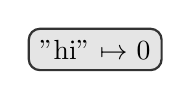
\begin{tikzpicture}
        [level distance=15mm,
        level 1/.style={sibling distance=36mm},
        level 2/.style={sibling distance=15mm},
        level 3/.style={sibling distance=12mm},
        ]
        \node[treenode] {\code{"hi"} $\mapsto$ \code{0}}
          child[missing]
          child[missing];
      \end{tikzpicture}
      \\ \code{T1}
    \end{center}
  \end{minipage}
  \begin{minipage}{0.49\textwidth}
    \begin{center}
      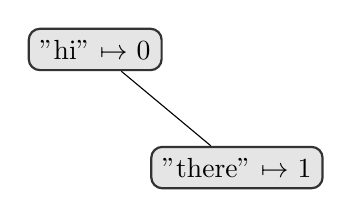
\begin{tikzpicture}
        [level distance=15mm,
        level 1/.style={sibling distance=36mm},
        level 2/.style={sibling distance=15mm},
        level 3/.style={sibling distance=12mm},
        ]
        \node[treenode] {\code{"hi"} $\mapsto$ \code{0}}
          child[missing]
          child{node[treenode] {\code{"there"} $\mapsto$ \code{1}}
            child[missing]
            child[missing]
          };
      \end{tikzpicture}
      \\ \code{T2}
    \end{center}
  \end{minipage}
\end{frame}

\begin{frame}[fragile]
  \frametitle{A Curious Comparison}

  Consider the following comparison function, however:
  \pause

  \begin{codeblock}
    fun to_pig_latin s =
      case String.explode s of
        [] => "ay"
      | c::cs => String.implode (cs @ [c]) ^ "ay"

    fun compare_pig_latin (s1, s2) =
      String.compare (to_pig_latin s1, to_pig_latin s2)
  \end{codeblock}

  \pause
  \vspace{\fill}

  This comparison function just compares two strings in Pig Latin\footnote{
    {\color{blue}\href{https://en.wikipedia.org/wiki/Pig_Latin}{See this reference for more}}
  } instead of
  in regular text.
\end{frame}

\begin{frame}[fragile]
  \frametitle{A Porcine Insertion}

  Notably, this is a valid comparison function of type \code{string * string -> order}!

  \pause
  \vspace{\fill}

  That means we can use it in conjunction with our \code{(string, int) Dict.t} trees
  that we defined earlier.

  \pause
  \vspace{\fill}

  \begin{codeblock}
    val T3 = Dict.insert compare_pig_latin ("class", 2) T2
  \end{codeblock}

  \pause
  \vspace{\fill}

  How does this insertion happen?
\end{frame}

\begin{frame}[fragile]
  \frametitle{A Porcine Insertion}

  \begin{minipage}[t]{0.4\textwidth}
    \begin{center}
      Inserting: \tikz[baseline] \node[treenode] {\code{"class"} $\mapsto$ 2};

      \vspace{40pt}

      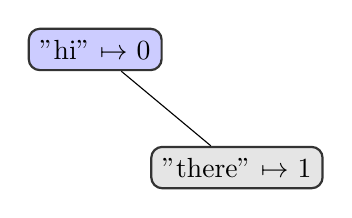
\begin{tikzpicture}
        [level distance=15mm,
        level 1/.style={sibling distance=36mm},
        level 2/.style={sibling distance=15mm},
        level 3/.style={sibling distance=12mm},
        ]
        \node[treenode, fill=blue!20!white] {\code{"hi"} $\mapsto$ \code{0}}
          child[missing]
          child{node[treenode] {\code{"there"} $\mapsto$ \code{1}}
            child[missing]
            child[missing]
          };
      \end{tikzpicture}

      \vspace{10pt}

      \code{T2}
    \end{center}
  \end{minipage}
  \begin{minipage}[t]{0.59\textwidth}
    \begin{center}
      Comparing: \\

      \vspace{20pt}

      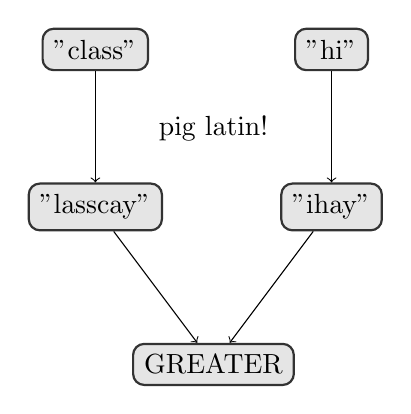
\begin{tikzpicture}
        \node[treenode] (T1) at (-1.5,3) {\code{"class"}};
        \node[treenode] (T2) at (1.5,3) {\code{"hi"}};

        \node[between=T1 and T2, yshift=-1cm] (P) {pig latin!};

        \node[treenode] (T3) at (-1.5,1) {\code{"lasscay"}};
        \node[treenode] (T4) at (1.5,1) {\code{"ihay"}};

        \node[treenode] (C) at (0,-1) {\code{GREATER}};
        \draw[<-] (T3) -- (T1);
        \draw[<-] (T4) -- (T2);
        \draw[<-] (C) -- (T3);
        \draw[<-] (C) -- (T4);
      \end{tikzpicture}
    \end{center}
  \end{minipage}
\end{frame}

\begin{frame}[fragile]
  \frametitle{A Porcine Insertion}

  \begin{minipage}[t]{0.4\textwidth}
    \begin{center}
      Inserting: \tikz[baseline] \node[treenode] {\code{"class"} $\mapsto$ 2};

      \vspace{40pt}

      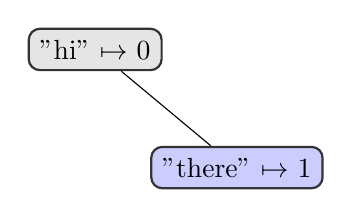
\begin{tikzpicture}
        [level distance=15mm,
        level 1/.style={sibling distance=36mm},
        level 2/.style={sibling distance=15mm},
        level 3/.style={sibling distance=12mm},
        ]
        \node[treenode] {\code{"hi"} $\mapsto$ \code{0}}
          child[missing]
          child{node[treenode, fill=blue!20!white] {\code{"there"} $\mapsto$ \code{1}}
            child[missing]
            child[missing]
          };
      \end{tikzpicture}

      \vspace{10pt}

      \code{T2}
    \end{center}
  \end{minipage}
  \begin{minipage}[t]{0.59\textwidth}
    \begin{center}
      Comparing: \\

      \vspace{20pt}

      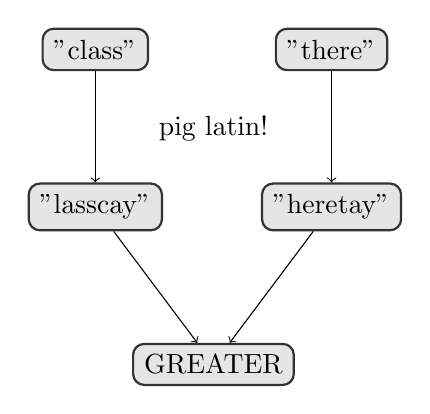
\begin{tikzpicture}
        \node[treenode] (T1) at (-1.5,3) {\code{"class"}};
        \node[treenode] (T2) at (1.5,3) {\code{"there"}};

        \node[between=T1 and T2, yshift=-1cm] (P) {pig latin!};

        \node[treenode] (T3) at (-1.5,1) {\code{"lasscay"}};
        \node[treenode] (T4) at (1.5,1) {\code{"heretay"}};

        \node[treenode] (C) at (0,-1) {\code{GREATER}};
        \draw[<-] (T3) -- (T1);
        \draw[<-] (T4) -- (T2);
        \draw[<-] (C) -- (T3);
        \draw[<-] (C) -- (T4);
      \end{tikzpicture}
    \end{center}
  \end{minipage}
\end{frame}

\begin{frame}[fragile]
  \frametitle{A Porcine Insertion}

  So finally, we end up with this tree:

  \pause
  \vspace{\fill}

  \begin{center}
    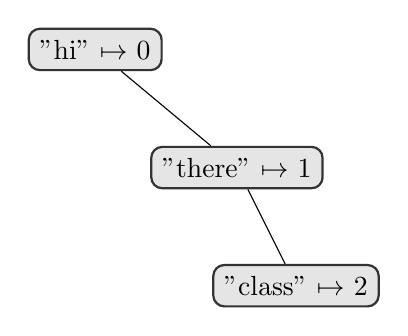
\begin{tikzpicture}
      [level distance=15mm,
      level 1/.style={sibling distance=36mm},
      level 2/.style={sibling distance=15mm},
      level 3/.style={sibling distance=12mm},
      ]
      \node[treenode] {\code{"hi"} $\mapsto$ \code{0}}
        child[missing]
        child{node[treenode] {\code{"there"} $\mapsto$ \code{1}}
          child[missing]
          child{node[treenode] {\code{"class"} $\mapsto$ \code{2}}
            child[missing]
            child[missing]
          }
        };
    \end{tikzpicture}

    \vspace{10pt}

    \code{T3}
  \end{center}

  \pause
  \vspace{\fill}

  Who sees an issue?
\end{frame}

\begin{frame}[fragile]
  \frametitle{A Classic Search}

  What happens if we try to look up the key \code{class} using our original
  \code{String.compare} function?

  \pause
  \vspace{\fill}

  \begin{center}
    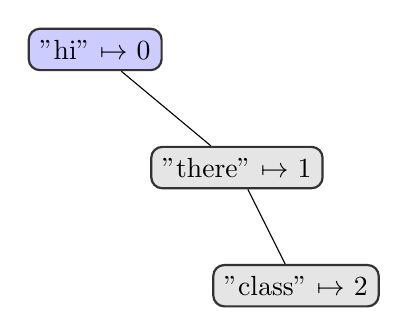
\begin{tikzpicture}
      [level distance=15mm,
      every node/.style={rounded corners, rectangle,inner sep=4pt, draw=black!80, thick},
      level 1/.style={sibling distance=36mm},
      level 2/.style={sibling distance=15mm},
      level 3/.style={sibling distance=12mm},
      ]
      \node[fill=blue!20!white] {\code{"hi"} $\mapsto$ \code{0}}
        child[missing]
        child{node[treenode] {\code{"there"} $\mapsto$ \code{1}}
          child[missing]
          child{node[treenode] {\code{"class"} $\mapsto$ \code{2}}
            child[missing]
            child[missing]
          }
        };
    \end{tikzpicture}

    \vspace{10pt}

    \code{T3}
  \end{center}

  \pause
  \vspace{\fill}

  Well, \code{String.compare ("class", "hi")} $\eeq$ \code{GREATER}, so:
\end{frame}

\begin{frame}[fragile]
  \frametitle{A Classic Search}

  \begin{center}
    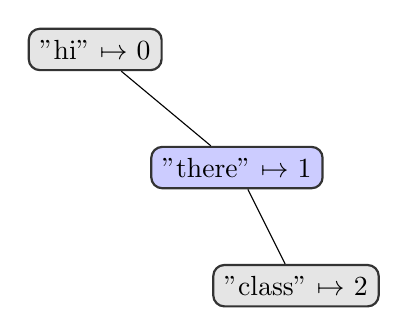
\begin{tikzpicture}
      [level distance=15mm,
      every node/.style={rounded corners, rectangle,inner sep=4pt, draw=black!80, thick},
      level 1/.style={sibling distance=36mm},
      level 2/.style={sibling distance=15mm},
      level 3/.style={sibling distance=12mm},
      ]
      \node[treenode] {\code{"hi"} $\mapsto$ \code{0}}
        child[missing]
        child{node[fill=blue!20!white] {\code{"there"} $\mapsto$ \code{1}}
          child[missing]
          child{node[treenode] {\code{"class"} $\mapsto$ \code{2}}
            child[missing]
            child[missing]
          }
        };
    \end{tikzpicture}

    \vspace{10pt}

    \code{T3}
  \end{center}

  \pause
  \vspace{\fill}

  And \code{String.compare ("class", "there")} $\eeq$ \code{LESS}.

  \pause
  \vspace{\fill}

  But, this means we need to go left, and the left node is \code{Empty}, so
  we don't find the mapping of \code{"class"} to \code{2} at all!

  \vspace{\fill}

  What went wrong?
\end{frame}

\begin{frame}[fragile]
  \frametitle{Mixing and Matching}

  The problem is that we mixed and matched our comparison functions.

  \pause
  \vspace{\fill}

  We originally had a tree which was a BST according to \code{String.compare},
  and then tried to insert a value into it as if it was a BST for our
  \code{compare_pig_latin} function!

  \pause
  \vspace{\fill}

  \customBox{Key Fact}{\, There is no \textit{static guarantee} that we give
  \code{Dict.lookup} and \code{Dict.insert} the same comparison functions.}

  \pause
  \vspace{\fill}

  We must merely exercise caution and care to make sure that we don't mix up our
  comparison functions. This sounds like a precondition -- but can we do better?
\end{frame}

\quizBreak{CATEGORICAL}

\sectionSlide{3}{Type Classes}

\begin{frame}[fragile]
  \frametitle{Concrete and Abstract}

  Signatures can either specify their types as \term{concrete types}, or leave
  them as \term{abstract types}, with definitions which are left to the
  structures that implement them. For instance, in the signature of
  \code{POLY_DICT}, the dictionary type \code{('a, 'b) t} was left abstract,
  because the implementation of dictionaries could be anything.

  \pause
  \vspace{\fill}

  We previously described opaque ascription as having the primary benefit of
  hiding the definitions of all involved abstract types, which helps in
  maintaining invariants and abstraction.

  \pause
  \vspace{\fill}

  Sometimes, we might still want to transparently ascribe to a signature, though.
  This is most salient with \term{type classes}.
\end{frame}

\begin{frame}[fragile]
  \frametitle{Type Classes}

  \defBox{}{A \term{type class} is the signature which describes a type,
  and some operations which may be performed on that type.}

  \pause
  \vspace{\fill}

  We use type classes to implement structures which ascribe to that type class,
  which witnesses the fact that some type supports that type class's operations.

  \pause
  \vspace{\fill}

  We call those structures which ascribe to a type class an \term{instance} of
  that type class.
\end{frame}

\begin{frame}[fragile]
  \frametitle{Type Classes}
  For instance, consider the following signature, which is a type class:
  \begin{codeblock}
    signature ORD =
      sig
        type t

        val compare : t * t -> order
      end
  \end{codeblock}

  \pause
  \vspace{\fill}

  This type class describes all types which admit a comparison function on them.
  Notably, this is a \textit{signature}, meaning that it is only a description
  that a module \textit{could} implement, but not an implementation itself!
\end{frame}

\begin{frame}[fragile]
  \frametitle{Orderable Types}

  Let's see some examples of implementations of the \code{ORD} signature:

  \pause
  \begin{codeblock}
    structure StrOrd : ORD =
      struct
        type t = string
        val compare = String.compare
      end

    structure IntOrd : ORD =
      struct
        type t = string
        val compare = Int.compare
      end
  \end{codeblock}
\end{frame}

\begin{frame}[fragile]
  \frametitle{Orderable Types}

  \begin{codeblock}
    structure PigLatinOrd : ORD =
      struct
        type t = string
        val compare = compare_pig_latin
      end
  \end{codeblock}

  \pause
  \vspace{\fill}

  Each of these structures are \term{instances} of the \code{ORD} type class,
  for a particular type!

  \pause
  \vspace{\fill}

  \noteBox{}{We choose to transparently ascribe these structures, because the
  point of a typeclass is that you know what the type inside of it is. I mean, it's
  in the name of the structure.}

  \pause
  \vspace{\fill}

  Note also how there can be multiple type classes for a single type, because there
  is not necessarily a single "canonical" kind of way to order a type. It depends
  on your context.
\end{frame}

\begin{frame}[fragile]
  \frametitle{A Generic Dictionary, v3}

  {\small
  \begin{codeblock}
    signature POLY_DICT =
      sig
        `structure Key : ORD`

        (* mapping keys of type Key.t to values of 'a *)
        type `'a` t

        val empty : 'a t
        val insert : `Key.t` * 'a -> 'a t -> 'a t
        val lookup : `Key.t` -> 'a t -> 'a option
      end
  \end{codeblock}
  }

  \pause
  \vspace{\fill}

  We make a third attempt at establishing a \code{POLY_DICT} signature.
  This time, instead of relying on doubly-parameterizing our dictionary
  type in the keys and values, we introduce an interior structure
  \code{Key}, which ascribes to the signature \code{ORD}.
\end{frame}

\begin{frame}[fragile]
  \frametitle{An Implementation for Polymorphic Dictionaries, v3}

  In essence, we are specifying that implementations of \code{POLY_DICT}
  should come packaged with an implementation of the \code{ORD} type class.
  In essence, we are localizing our comparison function to the one provided
  by \code{Key}!

  \pause
  \vspace{\fill}

  Here is one such implementation:

  \begin{codeblock}
    structure StrDict :> POLY_DICT =
      struct
        `structure Key = StrOrd`

        type `'a` t = `(Key.t * 'a)` tree

        val empty = Empty

      (* ... *)
  \end{codeblock}
\end{frame}

\begin{frame}[fragile]
  \frametitle{An Implementation for Polymorphic Dictionaries, v3}

  \small
  \begin{codeblock}
    (* ... *)
      fun insert (k, v) Empty = Node (Empty, (k, v), Empty)
        | insert (k, v) (Node (L, (k', v'), R)) =
            case `Key.compare` (k, k') of
              EQUAL   => Node (L, (k, v), R)
            | LESS    => Node (insert (k, v) L, (k', v'), R)
            | GREATER => Node (L, (k', v'), insert (k, v) R)

      fun lookup (k, v) Empty = NONE
        | lookup (k, v) (Node (L, (k', v'), R)) =
            case `Key.compare` (k, k') of
              EQUAL   => SOME v'
            | LESS    => lookup (k, v) L
            | GREATER => lookup (k, v) R
    end
  \end{codeblock}

  \pause
  \vspace{\fill}

  (We also got rid of the \code{cmp} functions, but it's hard to highlight the
  absence of something)
\end{frame}

\begin{frame}[fragile]
  \frametitle{Type Troubles}

  What happens if we try to actually use this implementation, however?

  \pause
  \vspace{\fill}

  \begin{mdframed}[leftmargin=0.5cm, roundcorner=10pt, backgroundcolor=black!86!white, rightmargin=0.5cm]
  \begin{center}
  \includegraphics[scale=0.5]{using_functor}
  \end{center}
  \end{mdframed}

  \pause
  \vspace{\fill}

  What gives? We defined the inner \code{Key} structure as \code{StrOrd}. Shouldn't
  this type-check?
\end{frame}

\begin{frame}[fragile]
  \frametitle{Too Opaque}
  {\small
  \begin{codeblock}
    signature POLY_DICT =
      sig
        structure Key : ORD

        (* mapping keys of type Key.t to values of 'a *)
        type 'a t

        val empty : 'a t
        val insert : `Key.t` * 'a -> 'a t -> 'a t
        val lookup : `Key.t` -> 'a t -> 'a option
      end
  \end{codeblock}
  }

  \pause
  \vspace{\fill}

  Recall that \code{StrDict} opaquely ascribes to this signature, \code{POLY_DICT}. This hides the
  type of \code{'a t}, as we wanted, but it also hides the type of \code{Key.t}! There's nothing
  here which tells us that \code{Key.t} is \code{string}.
\end{frame}

\begin{frame}[fragile]
  \frametitle{Selective Transparency}

  Fortunately, there is a mechanism in SML that lets us change a signature to one which
  is slightly more transparent, by explicitly defining some types, and making them no longer
  opaque.

  \pause
  \vspace{\fill}

  \defBox{}{We can modify a signature with \textit{selective transparency} by the syntax
  \code{SIG where type <name> = <type>}, which defines that the type
  named \code{<name>} is explicitly defined as the input \code{<type>}.}

  \pause
  \vspace{\fill}

  So, for instance, instead of writing \code{POLY_DICT}, we can write \code{POLY_DICT where type Key.t = string}
  to achieve the same signature, but where \code{Key.t} is explicitly \code{string}.
\end{frame}

\begin{frame}[fragile]
  \frametitle{An Implementation for Polymorphic Dictionaries, v4}

  Our new implementation looks very similar to the last, we just change one line:

  \pause
  \vspace{\fill}

  \begin{codeblock}
    structure StrDict :> POLY_DICT `where type Key.t = string` =
      struct
        structure Key = StrOrd

        type 'a t = (Key.t * 'a) tree

        val empty = Empty

        (* ... *)

      end
  \end{codeblock}

  \pause
  \vspace{\fill}

  That's it!
\end{frame}

\begin{frame}[fragile]
  \frametitle{Success}

  Now we can use the \code{StrDict} module, at the correct type.

  \pause
  \vspace{\fill}

  \begin{mdframed}[leftmargin=1cm, roundcorner=10pt, backgroundcolor=black!86!white, rightmargin=1cm]
  \begin{center}
  \includegraphics[scale=0.7]{using_functor2}
  \end{center}
  \end{mdframed}
\end{frame}

\begin{frame}[fragile]
  \frametitle{Generality?}

  But wait, all of this implementation was ultimately just specific to the
  \code{StrOrd} structure. This amounts to being exactly equivalent to our
  original dictionary, when we did dictionaries of only strings! What gives?

  \pause
  \vspace{\fill}

  We haven't really achieved generality, because we would have to write this
  text again for every single \code{Key} structure we are interested in using,
  like \code{IntOrd}, or \code{PigLatinOrd}, etc.

  \pause
  \vspace{\fill}

  If only there was some way we could parameterize our code on other modules.
\end{frame}

\sectionSlide{4}{Functors}

\begin{frame}[fragile]
  \frametitle{From Structure to Structure}

  We have seen an analogy where we have \term{structures}, which are groupings
  of values and other declarations, and which have a kind of \textit{"type"}, or
  interfaces, namely in the form of \term{signatures}.

  \pause
  \vspace{\fill}

  We can think of this as a correspondence between values and structures, which
  are described by types and signatures, respectively. We also have functions,
  which act as maps between values to values.

  \pause
  \vspace{\fill}

  Functors are the module analogue of functions, as maps from structures to structures.

  \vspace{\fill}

  \begin{center}
    \begin{tabular}{ c|c|c }
    Values & Types & Functions \\ [0.5ex]
    \hline & \\[-1.5ex]
    Structures & Signatures & Functors
    \end{tabular}
  \end{center}
\end{frame}

\begin{frame}[fragile]
  \frametitle{The Syntax of Functors}

  The syntax of functors is as follows:

  \begin{codeblock}
    functor Name (Arg : SIG) =
      struct
        (* ... *)
      end
  \end{codeblock}

  \pause
  \vspace{\fill}

  It looks similar to that of a \code{structure}, except a functor can take in
  a module. In this case, this declares a functor named \code{Name}, which takes
  in a module which it names \code{Arg}, so long as the input module ascribes to
  the signature \code{SIG}.

  \pause
  \vspace{\fill}

  This is analogous to a function declaration \code{fun name (arg : int) = (*
  ... *)}, which is named \code{name}, and takes in a value it names \code{arg},
  so long as the input value has type \code{int}.
\end{frame}

\begin{frame}[fragile]
  \frametitle{Ordering Pairs}

  One application of functors is in creating a functor which can create instances
  of the \code{ORD} type class out of other instances of the \code{ORD} type class.

  \pause
  \vspace{\fill}

  For instance, suppose we would like to order arbitrary tuples of two types,
  \code{t1} and \code{t2}. It would be annoying to have to write out, for every
  permutation of types,

  \pause
  \vspace{\fill}

  \begin{codeblock}
    structure IntStrOrd : ORD =
      struct
        type t = int * string

        fun compare ((i1, s1), (i2, s2)) =
          case Int.compare (i1, i2) of
            EQUAL   => String.compare (s1, s2)
          | LESS    => LESS
          | GREATER => GREATER
      end
  \end{codeblock}
\end{frame}

\begin{frame}[fragile]
  \frametitle{Composing Type Classes}

  \begin{codeblock}
    functor PairOrd (structure A : ORD
                     structure B : ORD) =
      struct
        type t = A.t * B.t

        fun compare ((a1, b1), (a2, b2)) =
          case A.compare (a1, a2) of
            EQUAL   => B.compare (b1, b2)
          | LESS    => LESS
          | GREATER => GREATER
      end
  \end{codeblock}

  \pause
  \vspace{\fill}

  This functor takes in two structures, \code{A} and \code{B}, both ascribing
  to \code{ORD}, and then does the natural left-to-right comparison of a
  tuple containing both, by leveraging the provided \code{A.compare} and
  \code{B.compare} functions.
\end{frame}

\begin{frame}[fragile]
  \frametitle{Composing Type Classes}

  \begin{codeblock}
    functor PairOrd (`structure A : ORD`
                     `structure B : ORD`) =
      struct
        type t = A.t * B.t

        fun compare ((a1, b1), (a2, b2)) =
          case A.compare (a1, a2) of
            EQUAL   => B.compare (b1, b2)
          | LESS    => LESS
          | GREATER => GREATER
      end
  \end{codeblock}

  \pause
  \vspace{\fill}

  But wait, what is going on in the highlighted region?
\end{frame}

\begin{frame}[fragile]
  \frametitle{Functorial Syntactic Sugar}

  Sometimes we are interested in a little more versatility in what our functor
  takes in. We might, for instance, want to take in a type and a value instead of
  just a module, or more than one structure.

  \pause
  \vspace{\fill}

  To that end, we can write the following syntax for a functor which takes in
  a type \code{t} and a value \code{x} of type \code{int}:

  \begin{codeblock}
    functor Name (type t
                  val x : int) =
      struct
        (* ... *)
      end
  \end{codeblock}

  \pause
  \vspace{\fill}

  \noteBox{}{There is no semicolon or comma between the two declarations of
  \code{type t} and \code{val x : int}. There's just space.}

  \pause
  \vspace{\fill}

  It is worth noting that this is just syntactic sugar, though!
\end{frame}

\begin{frame}[fragile]
  \frametitle{Functorial Syntactic Sugar}

  \noteBox{}{It is important to realize that a functor \textbf{can only take
  in one structure.}}

  \pause
  \vspace{\fill}

  This is no big issue, though, because structures themselves can contain types
  and values. The above syntax is really defining a functor \code{Name}, which
  takes in an \textbf{unnamed structure}, which ascribes to the signature

  \begin{codeblock}
    sig
      type t
      val x : int
    end
  \end{codeblock}

  \pause
  \vspace{\fill}

  We can, however, use the same syntactic sugar when calling the functor.

  \vspace{\fill}

  \begin{codeblock}
    structure Result = Name (type t = string
                             val x = 3)
  \end{codeblock}
\end{frame}

\begin{frame}[fragile]
  \frametitle{A Common Pitfall}

  It is important to realize this, because this means that our previous definition
  of \code{PairOrd} is really taking in a single structure, which contains two
  structures \code{A} and \code{B}!

  \pause
  \vspace{\fill}

  So in order to use it, we would write
  \begin{codeblock}
    structure IntStrOrd = PairOrd (structure A = IntOrd
                                   structure B = StrOrd)
  \end{codeblock}

  which will package both \code{IntOrd} and \code{StrOrd} into an unnamed
  module, which contains a module named \code{A} and \code{B}, which are just
  \code{IntOrd} and \code{StrOrd}.

  \pause
  \vspace{\fill}

  This can mess you up. The important thing to remember: \textbf{do not mix}
  syntactic sugar and not syntactic sugar! If you define a functor with syntactic
  sugar, you must call it using syntactic sugar.
\end{frame}

\begin{frame}[fragile]
  \frametitle{An Implementation for Polymorphic Dictionaries, v5}

  So now let's implement our polymorphic dictionaries, but now using this
  functor idea, so we can parameterize over all the possible key type classes.

  \pause
  \vspace{\fill}

  \begin{codeblock}
    `functor MkDict (Key : ORD)` :> POLY_DICT =
      struct
        structure Key = `Key`

        type 'a t = (Key.t * 'a) tree

        val empty = Empty

      (* ... *)
  \end{codeblock}
\end{frame}

\begin{frame}[fragile]
  \frametitle{An Implementation for Polymorphic Dictionaries, v5}

  {\small
  \begin{codeblock}
    (* ... *)
      fun insert (k, v) Empty = Node (Empty, (k, v), Empty)
        | insert (k, v) (Node (L, (k', v'), R)) =
            case Key.compare (k, k') of
              EQUAL   => Node (L, (k, v), R)
            | LESS    => Node (insert (k, v) L, (k', v'), R)
            | GREATER => Node (L, (k', v'), insert (k, v) R)

      fun lookup (k, v) Empty = NONE
        | lookup (k, v) (Node (L, (k', v'), R)) =
            case Key.compare (k, k') of
              EQUAL   => SOME v'
            | LESS    => lookup (k, v) L
            | GREATER => lookup (k, v) R
    end
  \end{codeblock}
  }

\end{frame}

\begin{frame}[fragile]
  \frametitle{Using Functors}

  Now, we can easily define dictionary structures by using our functor
  \code{MkDict}, like so:
  \pause

  \begin{codeblock}
    structure IntDict      = MkDict (IntOrd)
    structure StrDict      = MkDict (StrOrd)
    structure PigLatinDict = MkDict (PigLatinOrd)
  \end{codeblock}

  \pause
  \vspace{\fill}

  Much, much nicer.
\end{frame}

\begin{frame}[fragile]
  \frametitle{Using Functors}

  Now, we have the advantage that statically, \code{IntDict.t},
  \code{StrDict.t}, and \code{PigLatinDict.t} are all recognized as
  \textit{separate types}.

  \pause
  \vspace{\fill}

  Even though \code{StrDict.t} and \code{PigLatinDict.t} have the same
  representation on the inside, they cannot be mixed, and they use
  their own comparison functions independently of each other.

  \pause
  \vspace{\fill}

  Most critically, we avoid having to write intense amounts of boilerplate,
  and can (in a type-safe way) reuse our implementation of dictionaries,
  even though it was predicated on different types.

  \vspace{\fill}

  That's pretty cool!


\end{frame}

\begin{frame}[fragile]
  \frametitle{The Final Signature}
  \begin{codeblock}
    signature POLY_DICT =
      sig
        structure Key : ORD

        (* mapping keys of type Key.t to values of 'a *)
        type 'a t

        val empty : 'a t
        val insert : Key.t * 'a -> 'a t -> 'a t
        val lookup : Key.t -> 'a t -> 'a option
      end
  \end{codeblock}
\end{frame}
\begin{frame}[fragile]
  \frametitle{The Final Implementation}

  \tiny
  \begin{codeblock}
    functor MkDict (Key : ORD) :> POLY_DICT =
      struct
        structure Key = Key

        type 'a t = (Key.t * 'a) tree

        val empty = Empty

        fun insert (k, v) Empty = Node (Empty, (k, v), Empty)
          | insert (k, v) (Node (L, (k', v'), R)) =
              case Key.compare (k, k') of
                EQUAL   => Node (L, (k, v), R)
              | LESS    => Node (insert (k, v) L, (k', v'), R)
              | GREATER => Node (L, (k', v'), insert (k, v) R)

        fun lookup (k, v) Empty = NONE
          | lookup (k, v) (Node (L, (k', v'), R)) =
              case Key.compare (k, k') of
                EQUAL   => SOME v'
              | LESS    => lookup (k, v) L
              | GREATER => lookup (k, v) R
      end
  \end{codeblock}
\end{frame}

% \begin{frame}[plain]
% 	\begin{center} Thank you! \end{center}

% 	\begin{center}
%     {\color{blue} \href{https://docs.google.com/forms/d/e/1FAIpQLSfAjJB9M1Jt-AV_290144DaRvzkjqXklQ4Q3OL7lDIic3nx2g/viewform?usp=sf_link}{Post-lecture survey:}} \\
%     \vspace{5pt}
%     \includegraphics[scale=0.035]{qr_july11} \\
%     \vspace{5pt}
%     And the House Quiz winner is...
%   \end{center}
% \end{frame}

\thankyou

\end{document}